\chapter{Aportaciones}

\section{Redes Neuronales Totalmente Conectadas}

\subsection{Gradiente de la función de pérdida respecto a SoftMax, \cite{Cross_entropy_backprop} \cite{Cross_entropy_backprop_grad_input}} 

Siendo $Z_i$ la salida de la neurona $n_i$ de la última capa oculta, se denotará como $O_i$ una vez pase por la capa softmax. \\

\begin{figure}[H]
	\centering
	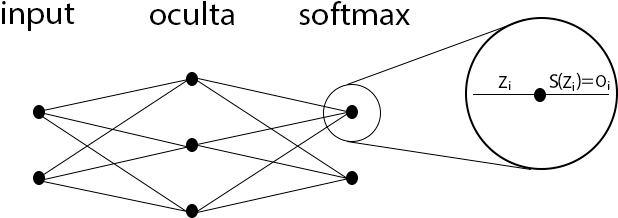
\includegraphics[scale=0.4]{imagenes/NN_softmax.jpg}  
	\caption{Estructura de una red con softmax}
\end{figure}

\begin{gather}
	E = - \sum_{i=1}^{H}  [y_i * log(O_i)] 
	\label{cross_entropy_notacion}
\end{gather}

Según esta notación, la función de error \ref{loss_func_softmax} se convierte en la fórmula \ref{cross_entropy_notacion}.

\subsubsection{Gradiente de la función de error}

\begin{gather}
	\frac{\partial E}{\partial Z_k} = \frac{\partial(- \sum_{i=1}^{H}  [y_i * log(O_i)])}{\partial Z_k} = - \sum_{i=1}^{H}  [\frac{\partial(y_i * log(O_i))}{\partial Z_k}] 
\end{gather}

Como $y_i$ es independiente respecto a $Z_k$, se trata como una constante. \\
\begin{gather}
	\frac{\partial E}{\partial Z_k} = - \sum_{i=1}^{H}  [y_i * \frac{\partial(log(O_i))}{\partial Z_k}] 
\end{gather}

Se aplica la regla de la cadena, pues $O_i$ no depende directamente de $Z_k$,. \\
\begin{gather}	
	\frac{\partial E}{\partial Z_k} = - \sum_{i=1}^{H}  [y_i * \frac{\partial(log(O_i))}{\partial O_i} * \frac{\partial O_i}{\partial Z_k}] \\
	\frac{\partial E}{\partial Z_k} = - \sum_{i=1}^{H}  [\frac{y_i}{O_i} * \frac{\partial O_i}{\partial Z_k}] 
	\label{gradiente_Oi_Zk}
\end{gather}

% ver https://www.mldawn.com/the-derivative-of-softmaxz-function-w-r-t-z/

\subsubsection{Derivada de softmax respecto de su entrada, $\frac{\partial O_i}{\partial Z_k}$}

Hay 2 casos posibles, $\frac{S(Z_i)}{Z_i}$ o $\frac{S(Z_i)}{Z_j}$, donde i $\neq$ j. \\

\subsubsection{Caso $\frac{S(Z_i)}{Z_i}$}

\begin{gather}
	\frac{\partial f(x)}{\partial g(x)} = \frac{f'(x)*g(x) - g'(x)*f(x)}{g(x)^2} \\
	S(z_i) = \frac{e^{Z_i}}{e^{Z_1} + ... + e^{Z_H}} \\
	\frac{\partial S(Z_1)}{\partial Z_1} = \frac{[\frac{\partial e^{Z_1}}{\partial Z_1} * (e^{Z_1} + ... + e^{Z_H}) ] - [\frac{\partial (e^{Z_1} + ... + e^{Z_H})}{\partial Z_1} * e^{Z_1} ] }{(e^{Z_1} + ... + e^{Z_H})^2} 
\end{gather}

Se aplica $\frac{\partial e^{Z_1}}{Z_1} = e^{Z_1}$ \\
\begin{gather}
	\frac{\partial S(Z_1)}{\partial Z_1} = \frac{[e^{Z_1} * \sum_{i=1}^{H}  e^{Z_i}] - [e^{Z_1} * e^{Z_1}]   }{ (\sum_{i=1}^{H}  e^{Z_i})^2} \\
\end{gather}

Se saca factor común $e^{Z_1}$ \\
\begin{gather}
	\frac{\partial S(Z_1)}{\partial Z_1} = \frac{e^{Z_1} ([\sum_{i=1}^{H}  e^{Z_i}] - e^{Z_1})  }{(\sum_{i=1}^{H}  e^{Z_i})^2} \\
	\frac{\partial S(Z_1)}{\partial Z_1} = \frac{e^{Z_1}}{\sum_{i=1}^{H}  e^{Z_i}} * \frac{[\sum_{i=1}^{H}  e^{Z_i}] - e^{Z_1}}{\sum_{i=1}^{H}  e^{Z_i}}
\end{gather}

Se recuerda que $\frac{\sum_{i=1}^{H}  e^{Z_i}}{\sum_{i=1}^{H}  e^{Z_i}} = 1$ y que S($Z_1$) = $ \frac{e^{Z_1}}{\sum_{i=1}^{H}  e^{Z_i}}$ \\
\begin{gather}
	\frac{\partial S(Z_1)}{\partial Z_1} = S(Z_1) * (1- S(Z_1))
	\label{grad_Oi_Zk_drch}
\end{gather}

\subsubsection{Caso $\frac{S(Z_i)}{Z_j}$, con i $\neq$ j}

\begin{gather}
	\frac{\partial S(Z_2)}{\partial Z_1} = \frac{[\frac{\partial e^{Z_2}}{\partial Z_1} * (e^{Z_1} + ... + e^{Z_H}) ] - [\frac{\partial (e^{Z_1} + ... + e^{Z_H})}{\partial Z_1} * e^{Z_2} ] }{(e^{Z_1} + ... + e^{Z_H})^2} \\
	\frac{\partial S(Z_2)}{\partial Z_1} = \frac{[0 * [\sum_{i=1}^{H}  e^{Z_i}]] - [e^{Z_1} * e^{Z_2}]   }{ (\sum_{i=1}^{H}  e^{Z_i})^2} \\
	\frac{\partial S(Z_2)}{\partial Z_1} = \frac{-e^{Z_1} * e^{Z_2}  }{(\sum_{i=1}^{H}  e^{Z_i})^2} \\
	\frac{\partial S(Z_2)}{\partial Z_1} = \frac{-e^{Z_1}}{\sum_{i=1}^{H}  e^{Z_i}} * \frac{e^{Z_2}}{\sum_{i=1}^{H}  e^{Z_i}} \\
	\frac{\partial S(Z_2)}{\partial Z_1} = -S(Z_1) * S(Z_2)
	\label{grad_Oi_Zk_izq}
\end{gather}

\subsubsection{Combinación de casos}

De esta forma, tendremos que dividir  el proceso en 2 partes, cuando i sea igual a j, y cuando i $\neq$ j, perteneciendo a la primera todos los casos menos uno. \\
Parte izquierda cuando i!=k, parte derecha cuando i=k. \\
Retomamos la fórmula \ref{gradiente_Oi_Zk}, aplicando \ref{grad_Oi_Zk_izq} en la parte izquierda y \ref{grad_Oi_Zk_drch} en la derecha. \\
\begin{gather}
	\frac{\partial E}{\partial Z_k} = - [\sum_{i!=k}^{H} [\frac{y_i}{O_i} * -O_i * O_k ] + \frac{y_k}{O_k} * O_k * (1 - O_k)  ]
\end{gather}

Se simplifica $O_i$ en la parte izquierda y $O_k$ en la derecha. \\
\begin{gather}
	\frac{\partial E}{\partial Z_k} = - [\sum_{i!=k}^{H} [- y_i * O_k] + [y_k * (1 - O_k) ] ] 
\end{gather}

Se extrae $O_k$ de la suma, pues es independiente respecto al índice $i$ \\
\begin{gather}	
	\frac{\partial E}{\partial Z_k} = - [-O_k \sum_{i!=k}^{H}- y_i + [y_k * (1 - O_k) ] ]
	\label{simplificar}
\end{gather}

\subsubsection{Simplificación One-Hot}

Al emplear la codificación one-hot en Y, se sabe que la suma de sus elementos es igual a 1. \\
\begin{gather}
	\sum_{i=1}^{H} y_i = 1 \\
	\sum_{i!=k}^{H} y_i = \sum_{i=1}^{H} y_i - y_k = 1 - y_k
	\label{one_hot_simplif}
\end{gather}

Se emplea \ref{one_hot_simplif} para simplificar la suma en \ref{simplificar}. \\


\begin{gather}
	\frac{\partial E}{\partial Z_k} = [O_k*(1-y_k)] - [y_k*(1-O_k)] \\
	\frac{\partial E}{\partial Z_k} = O_k - O_k * y_k - y_k + O_k * y_k 
\end{gather}

Se simplifica $O_k*y_k$. \\
\begin{gather}
	\frac{\partial E}{\partial Z_k} = O_k - y_k
\end{gather}

\subsection{BackPropagation con 1 capa oculta}

\begin{figure}[H]
	\centering
	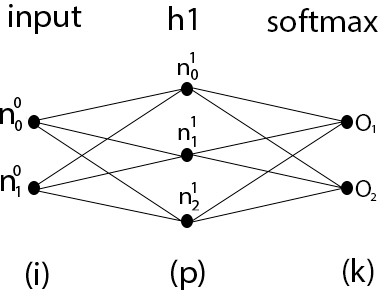
\includegraphics[scale=0.35]{imagenes/nn_1_capa.jpg}  
	\caption{Red Neuronal totalmente conectada con 1 capa oculta}
	\label{fig:nn_1_capa}
\end{figure}

La Figura 3.1 se compone de puntos y líneas, representando neuronas y pesos que las conectan respectivamente. Cada punto es una neurona, y cada línea un peso. \\
La Figura \ref{fig:nn_1_capa} presenta 3 capas (input, h1, output) que corresponden a capa de entrada, capa oculta $h_1$, y capa de salida respectivamente. El superíndice indica la capa a la que pertenece una neurona o peso, mientras que el subíndice indica el número del mismo en su respectiva capa. En el caso de los pesos, se requieren 2 subíndices para identificar a cada uno (pues un peso une 2 neuronas). \\
La capa de entrada se compone de 2 neuronas ($n^{0}_0$ y $n^{0}_1$). \\
La capa oculta $h_1$ tiene 3 neuronas ($n^1_{0}$, $n^1_{1}$, y $n^1_{2}$) \\
El peso $W^{i}_{jk}$ referencia al peso que une las neuronas $n^{i}_j$ y $n^{i+1}_k$.\\
Además, se denotará como $\hat{y}$ a la última neurona de la red, pues contendrá la predicción de la misma.  

\subsubsection{Capa output}

\begin{figure}[H]
	\centering
	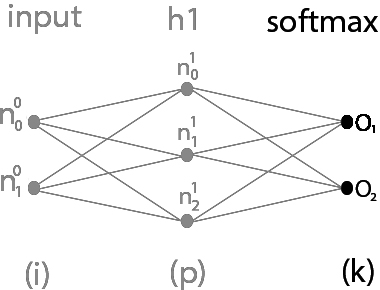
\includegraphics[scale=0.35]{imagenes/nn_1_capa_output.jpg}  
	\caption{Imagen de backpropagation en la capa output}
	\label{fig:nn_1_capa_output}
\end{figure}

Sea la neurona $n^i_j$, se define como $a^i_j$ el valor de dicha neurona antes de aplicar sobre ella su función de activación asociada, y $z^i_j$ el obtenido tras aplicarla. De forma adicional, se usará $\hat{a}$ y $\hat{z}$ para $\hat{y}$.

Así, la función de pérdida \ref{loss_func} se convierte en:

\begin{gather}
	H(x) = - \frac{1}{N} \sum_{i=1}^{N}  [y_i * log( \hat{z}_i) + (1-y_i)*log(1-\hat{z}_i)]
	\label{loss_func_az}
\end{gather}

Para realizar el descenso del gradiente, se debe empezar calculando la derivada de la función de pérdida respecto a la predicción obtenida. Es decir, la derivada de la fórmula (3.1) respecto de las neuronas en la última capa de la red tras aplicar sus respectivas funciones de activación, que en este caso corresponde a $\hat{z}$. \\
Por simplicidad, podemos dividir esta derivada en 2 partes. \\
Parte izquierda:
\begin{gather}
	f(x) = A*B \\  
	f'(x) = AB' + A'B \\
	\frac{\partial y_i}{\partial \hat{z}_i} = 0 \\
	\frac{\partial log(\hat{z}_i)}{\partial \hat{z}_i} = \frac{1}{\hat{z}_i} \\
	\frac{\partial y_i * log( \hat{z}_i)}{\partial \hat{z}_i} = y_i*\frac{1}{\hat{z}_i} + 0*log(\hat{z}_i) = \frac{y_i}{\hat{z}_i}
\end{gather}

Parte derecha:
\begin{gather}
	\frac{\partial (1-y_i)}{\partial \hat{z}_i} = 0\\
	\frac{\partial log(1-\hat{z}_i)}{\partial \hat{z}_i} = \frac{1}{1-\hat{z}_i} * (-1) \\
	\frac{\partial (1-y_i)*log(1-\hat{z}_i)}{\partial \hat{z}_i} = (1-y_i)*\frac{1}{1-\hat{z}_i}*(-1) + 0* log(1-\hat{z}_i) \\
	\frac{\partial (1-y_i)*log(1-\hat{z}_i)}{\partial \hat{z}_i} = -\frac{1-y_i}{1-\hat{z}_i}
\end{gather}

Finalmente, se obtiene: 
\begin{gather}
	\frac{\partial H(x)}{\partial \hat{z}_i} = - \frac{1}{N} \sum_{i=1}^{N}  [ \frac{y_i}{\hat{z}_i} - \frac{1-y_i}{1-\hat{z}_i} ]
\end{gather}

\subsubsection{Función activación de la capa output}
En la capa output se emplea la función de activación sigmoide. 

\begin{gather}
	sigmoide(x) = \frac{1}{1+e^{-x}} \\
	sigmoide'(x) = \frac{sigmoide(x)}{1-sigmoide(x)}
\end{gather}

De esta forma,

\begin{gather}
	\frac{\partial \hat{z}}{\partial \hat{a}} = \frac{\partial sigmoide(\hat{a})}{\partial \hat{a}} = sigmoide(\hat{a})*(1-sigmoide(\hat{a}))
\end{gather}

Ahora, podemos calcular el gradiente completo hasta la capa output antes de aplicar su función de activación.

\begin{gather}
	grad\_output = \frac{\partial H(x)}{\partial \hat{z}} * \frac{\partial \hat{z}}{\partial \hat{a}} =
	- \frac{1}{N} \sum_{i=1}^{N}  [ \frac{y_i}{\hat{z}_i} - \frac{1-y_i}{1-\hat{z}_i} ] * \frac{\partial \hat{z}}{\partial \hat{a}} \\
	grad\_output = - \frac{1}{N} \sum_{i=1}^{N}  [ \frac{y_i}{\hat{z}_i} - \frac{1-y_i}{1-\hat{z}_i} ] * sigmoide(\hat{a})*(1-sigmoide(\hat{a}))
\end{gather}

\subsubsection{Pesos capas h1-output}

\begin{figure}[H]
	\centering
	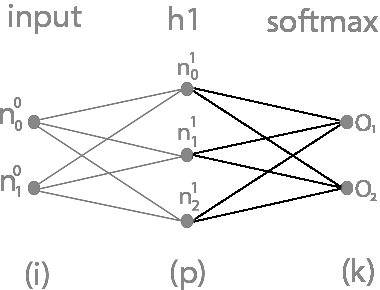
\includegraphics[scale=0.35]{imagenes/nn_1_capa_pesos_h1_output.jpg}  
	\caption{Imagen de backpropagation en los pesos entre la capa oculta y la capa output}
	\label{fig:nn_1_pesos_h1_output}
\end{figure}

Una vez calculado el gradiente hasta la capa output, se puede calcular el gradiente respecto a cada peso que se encuentra conectado a esta desde la capa anterior. Es decir, para cada $h^1_p\in h_1$, se calcula $\frac{dH(x)}{dW^1_{p\hat{y}}}$. Usando la regla de la cadena, equivale a realizar lo siguiente:

\begin{gather}
	\frac{\partial \hat{y}}{\partial W^1_{p\hat{y}}} = \frac{\partial n^1_p * W^1 _{p\hat{y} }}{\partial W^1_{p\hat{y} }} = n^1_p \\
	\frac{\partial H(x)}{\partial W^1_{p\hat{y} }} = \frac{\partial H(x)}{\partial \hat{y}} * \frac{\partial\hat{z}}{\partial \hat{a}} * \frac{\partial \hat{y}}{\partial W^1_{p\hat{y} }} =  grad\_output * \frac{\partial \hat{y}}{\partial W_{p\hat{y} }} = grad\_output * n^1_p
\end{gather}

\subsubsection{Capa oculta h1}

\begin{figure}[H]
	\centering
	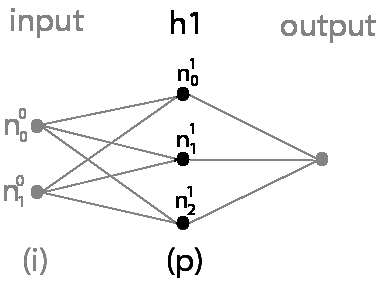
\includegraphics[scale=0.35]{imagenes/nn_1_capa_h1.jpg}  
	\caption{Imagen de backpropagation en la capa oculta h1}
	\label{fig:nn_1_capa_h1}
\end{figure}

\begin{gather}
	\frac{\partial \hat{y}}{\partial n^1_p} = \frac{\partial n^1_p * \partial W^1 _{p\hat{y}} }{\partial n^1_p } = \partial W^1_{p\hat{y}} \\
	deriv\_relu(x) = 0\ si\ x <= 0,\ 1\ en\ caso\ contrario \\
	\frac{\partial z^1_p }{\partial a^1_p } = \frac{\partial relu(a^1_p)}{\partial a^1_p } = deriv\_relu(a^1_p) \\
	\frac{\partial H(x) }{\partial n^1_p } = grad\_output* \frac{\partial \hat{y} }{\partial n^1_p } * \frac{\partial z^1_p }{\partial a^1_p } = grad\_output * W^1_{p\hat{y} } * deriv\_relu(a^1_p ) \\
	\frac{\partial H(x) }{\partial n^1_p } = gradient\_n^1_p
\end{gather}

\subsubsection{Pesos capas input-h1}

\begin{figure}[H]
	\centering
	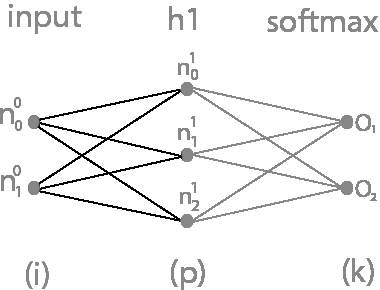
\includegraphics[scale=0.35]{imagenes/nn_1_capa_pesos_input_h1.jpg}  
	\caption{Imagen de backpropagation en los pesos entre la capa input y la capa oculta}
	\label{fig:nn_1_pesos_input_h1}
\end{figure}


\begin{gather}
	\frac{\partial n^1_p }{\partial W^0_{ip} } = \frac{\partial n^0_i * W^0_{ip} }{\partial W^0_{ip} } = n^0_i \\
	\frac{\partial H(x) }{\partial W^0_{ip} } = gradient\_n^1_p * \frac{\partial n^1_p }{\partial W^0_{ip} } = gradient\_n^1_p * n^0_i 
\end{gather}


\subsubsection{Capa input}

\begin{figure}[H]
	\centering
	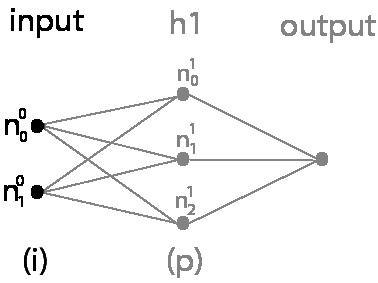
\includegraphics[scale=0.35]{imagenes/nn_1_capa_input.jpg}  
	\caption{Imagen de backpropagation en la capa input}
	\label{fig:nn_1_capa_input}
\end{figure}

\begin{gather}
	\frac{\partial n^1_p }{\partial n^0_i } = \frac{\partial n^0_i * W^0_{ip} }{\partial n^0_i } = W^0_{ip} \\
	\frac{\partial z^0_i }{\partial a^0_i } = 1
\end{gather}

Ahora se realiza una sumatoria con todos los 'caminos posibles' hacia la misma neurona
\begin{gather}
	\frac{\partial H(x) }{\partial n^0_i } = \sum_{p=0}^{h_1.size()} gradient\_n^1_p * \frac{\partial n^1_p }{\partial n^0_i } * \frac{\partial z^0_i }{\partial a^0_i }  \\
	\frac{\partial H(x) }{\partial n^0_i } = \sum_{p=0}^{h_1.size()}  gradient\_n^1_p * W^0_{ip}
\end{gather}

